\section{Experiments and Results}
We use transactional data from instacart kaggle challenge to train all our models. A preview of data used is 
shown in Figure~\ref{fig:sampledata}. 

 \begin{figure}[t]
    \centering 
    \caption{Sample Dataset} 
    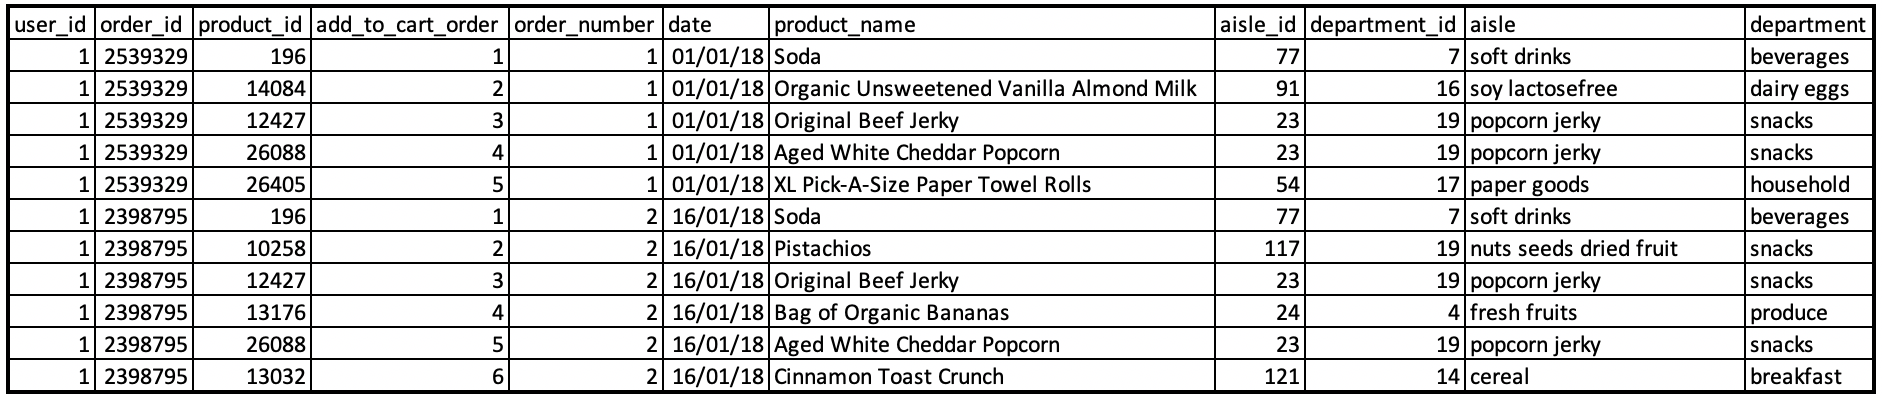
\includegraphics[width=3.3in]{img/sampledata.png} 
    \label{fig:sampledata} 
  \end{figure}

  \begin{figure}[t]
    \centering 
    \caption{Most ordered Items across Departments} 
    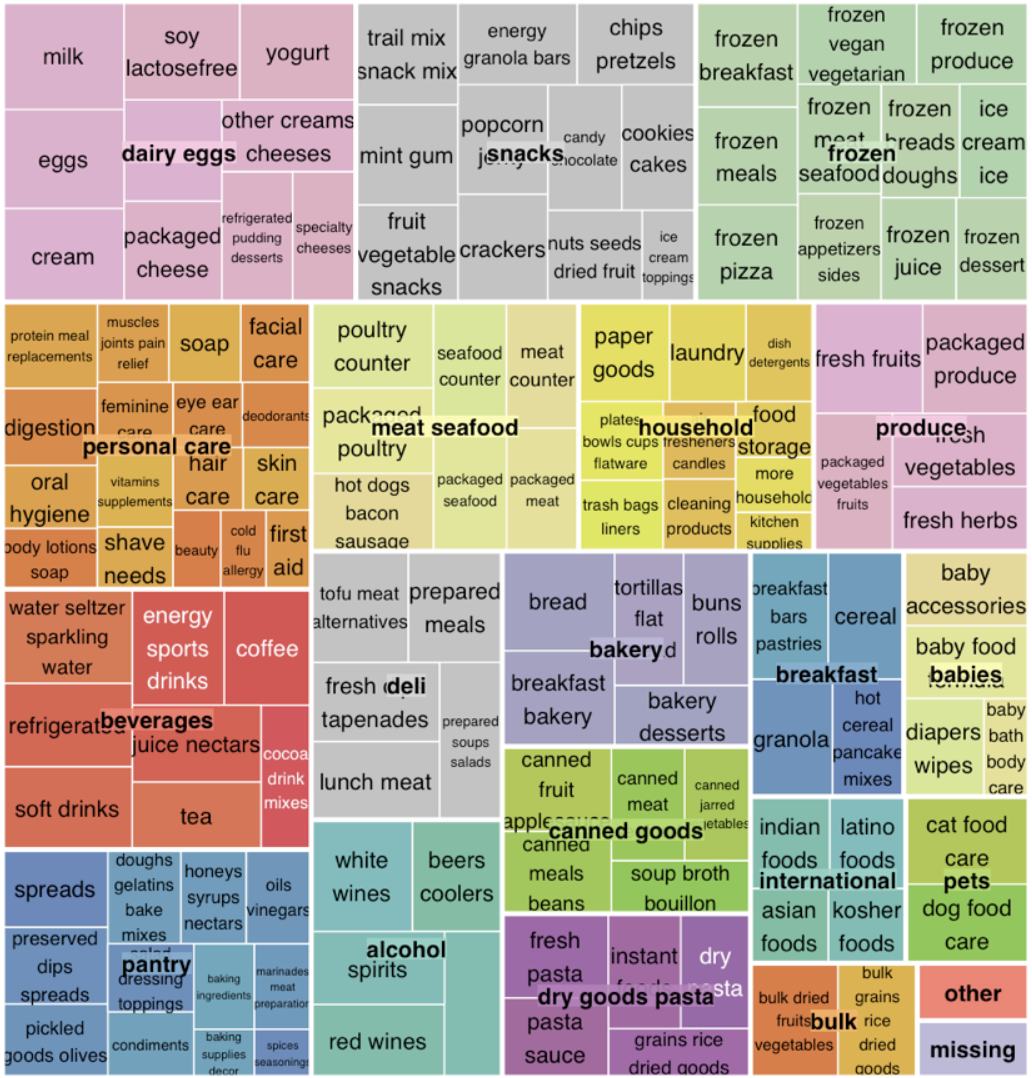
\includegraphics[width=3.3in]{img/items.png} 
    \label{fig:items} 
  \end{figure}

  \begin{figure}[t]
    \centering 
    \caption{Density of consumers Vs. Basket Size} 
    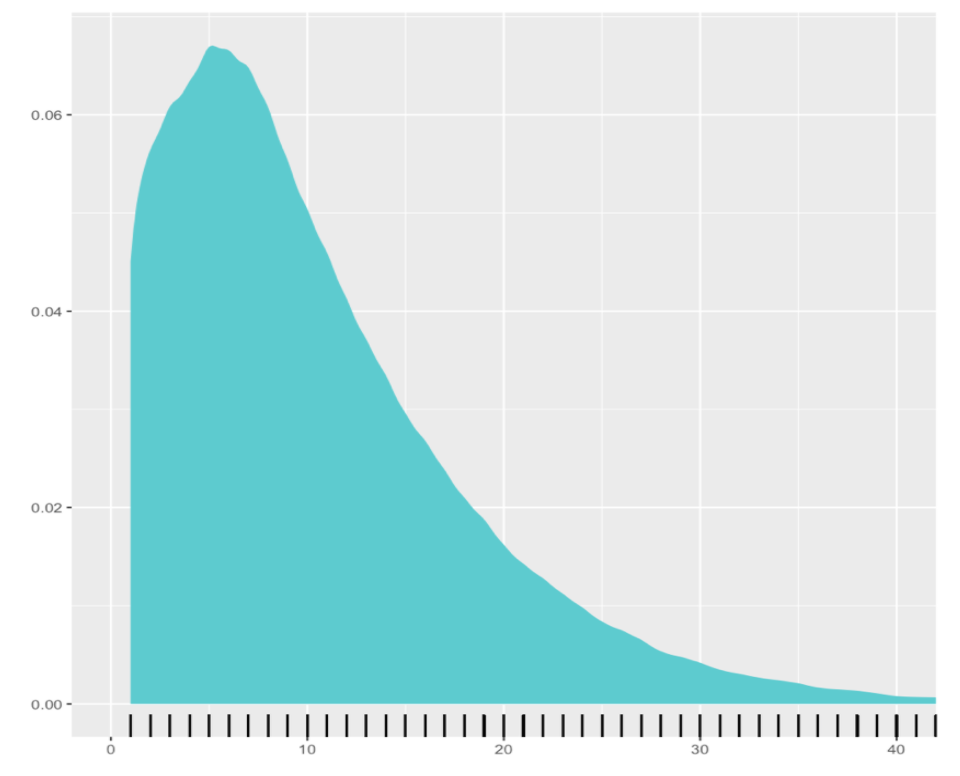
\includegraphics[width=3.3in]{img/basket.png} 
    \label{fig:basket} 
  \end{figure}

  \begin{figure}[t]
    \centering 
    \caption{Order probability Vs. Add to cart order} 
    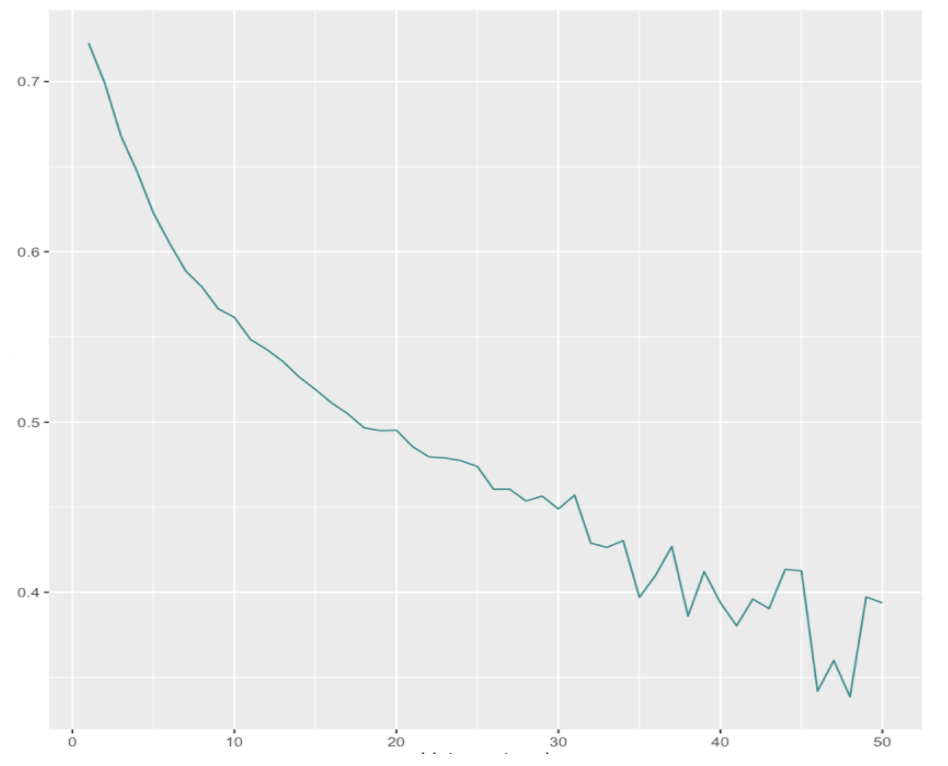
\includegraphics[width=3.3in]{img/addtocart.png} 
    \label{fig:basket} 
  \end{figure}

\begin{center}
\begin{table*}[!t]
\caption{BCELoss of Test2 for 12 Trials of Deep Learning Models} 
\centering
\resizebox{\textwidth}{!}{\begin{tabular}{|r|l|r|r|r|r|r|r|r|}
  \hline
 {\bf Trial} & {\bf Optimizer} & {\bf Scheduler} & {\bf SWA} & {\bf Parameter Avg} &  {\bf MLP} & {\bf LSTM} 
 &  {\bf TCN} & {\bf TCN-LSTM} \\ [0.5ex] 
  \hline\hline
1 & RMSprop & ReduceLROnPlateau & True & False &  10 & 0.52 & 0.67 & 0.30 \\ 
2 & RMSprop & CyclicLR & True & False &  54 & 0.55 & 0.64 & 0.25 \\ 
3 & Adam & ReduceLROnPlateau & True & False &  17 & 0.38 & 0.61 & 0.13 \\ 
4 & RMSprop & ReduceLROnPlateau & False & False &  10 & 0.52 & 0.62 & 0.28 \\ 
5 & RMSprop & CyclicLR & False & False &  10 & 0.53 & 0.66 & 0.27 \\ 
6 & Adam & ReduceLROnPlateau & False & False&  13 & 0.61 & 0.74 & 0.26 \\ 
7 & RMSprop & ReduceLROnPlateau & False & True &  44 & 0.55 & 0.48 & 0.12 \\ 
8 & RMSprop & CyclicLR& False & True &  10 & 0.66 & 0.73 & 0.27 \\ 
9 & Adam & ReduceLROnPlateau & False & True & 121 & 0.44 & 0.49 & 0.16 \\ 
10 & RMSprop & ReduceLROnPlateau & True & True & 158 & 0.72 & 0.73 & 0.17 \\ 
11 & RMSprop & CyclicLR & True & True &  11 & 0.69 & 0.70 & 0.18 \\ 
12 & Adam  & ReduceLROnPlateau & True & True&  19 & 0.67 & 0.65 & 0.14 \\ [1ex] 
   \hline
\end{tabular}}
\end{table*} 
\end{center}

\begin{table}[t]
\caption{BCELoss of Test2 for 6 best Trials of ML Models}
\vspace{0.1 in}
\centering
\resizebox{3.3in}{!}
{%
\begin{tabular}{|c|c|c|c|c|}
\hline
{\bf Trial} & {\bf Hyper-Parameter} & {\bf Xgboost} & {\bf RandomForest} \\  
\hline\hline
1  		&  Bayesian-Optimizer &  0.18 &  0.18   \\ 
2	  		&  Bayesian-Optimizer &  0.18 &  0.18   \\ 
3  		&  Bayesian-Optimizer &  0.18 &  0.18  \\ 
4	  		&  Bayesian-Optimizer &  0.18 &  0.18  \\ 
5	  		&  Bayesian-Optimizer &  0.18 &  0.18  \\ 
6	  		&  Bayesian-Optimizer &  0.18 &  0.18  \\ 
\hline
\end{tabular}
}
\label{tab:mlmodels}
\end{table}


\begin{table}[t]
\caption{ Training Results}
\vspace{0.1 in}
\centering
\resizebox{3.3in}{!}
{%
\begin{tabular}{|c|c|c|c|c|}
\hline
{\bf Model Type} & {\bf Train BCELoss} & {\bf Val BCELoss} & {\bf Test1 BCELoss} & {\bf Test2 BCELoss} \\ 
\hline\hline 
MLP	  		&  0.18 &  0.18 &  0.18 &  0.18  \\ \hline
LSTM  		&  0.18 &  0.17 &  0.17 &  0.17 \\ \hline
TCN			&  0.18 &  0.15  &  0.15 &  0.15  \\ \hline
TCNLSTM 	&  0.18 & 0.13  & 0.13	& 0.13	 \\ \hline
Xgboost 	&  0.18 & 0.21 & 0.21	& 0.21	\\ \hline
RandomForest &  0.18 & 0.23 & 0.23	& 0.23	\\ \hline
\end{tabular}
}
\label{tab:training}
\end{table}


\begin{table}[t]
\caption{ Stacked Generalization Results}
\vspace{0.1 in}
\centering
\resizebox{3.3in}{!}
{%
\begin{tabular}{|c|c|c|c|c|c|}
\hline
{\bf Model Type} & {\bf K Value} & {\bf Train BCELoss} & {\bf Val BCELoss} & {\bf Test1 BCELoss} & {\bf Test2 BCELoss} \\ 
\hline\hline 
Weighted K Best	  		&  5 &  0.18  &  0.18 &  0.18 &  0.18  \\ \hline
Weighted K Best	  		&  10 &  0.18  &  0.18 &  0.18 &  0.18  \\ \hline
Weighted K Best	  		&  25 &  0.18  &  0.18 &  0.18 &  0.18  \\ \hline
K Best	  		&  3 &   0.18 & 0.18 &  0.18 &  0.18  \\ \hline
K Best	  		&  5 &  0.18  &  0.18 &  0.18 &  0.18  \\ \hline
\end{tabular}
}
\label{tab:stacking}
\end{table}

\begin{table}[t]
\caption{Final Accuracy post F\textsubscript{1}-Maximization}
\vspace{0.1 in}
\centering
\resizebox{3.3in}{!}
{%
\begin{tabular}{|c|c|c|c|}
\hline
{\bf Data Split} & {\bf Precision} & {\bf Recall} & {\bf F\textsubscript{1}-Score} \\ 
\hline\hline 
Train	  		 &  0.18 &  0.18 &  0.18  \\ \hline
Validation	  	 &  0.18 &  0.18 &  0.18  \\ \hline
Test1	  		 &  0.18 &  0.18 &  0.18  \\ \hline
Test2	  		 & 0.18 &  0.18 &  0.18  \\ \hline
\end{tabular}
}
\label{tab:Fscore}
\end{table}